\Large\textbf{\textcolor{blue}{5.  *Punto extra*}} 
Observa la siguiente función del lenguaje de programación \code{Racket}

\begin{lstlisting}
(let ([sum (lambda (n) (if (zero? n) 0 (+ n (sum (sub1 n))))))])
      (sum 5))
\end{lstlisting}

\begin{enumerate}[a.]
%%%%%%%%%%%%%%%%%%%%%%%%%%%%%      Inciso A        %%%%%%%%%%%%%%%%%%%%%%%%%%%%%%%%%
\item Prueba la expresión en el intérprete de \code{Racket} y con base en la respuesta 
obtenida, explica el proceso que siguió el intérprete para llegar a ésta. Anexa una 
captura de pantalla del intérprete de \code{Racket} al probar la expresión.

\begin{figure}[h]
  \centering
  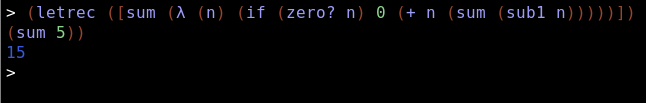
\includegraphics[scale=0.5]{./Sum.png}
  \caption{Ejecución de la función dada.}
\end{figure}

\begin{lstlisting}
> (let ([sum (lambda (n) (if (zero? n) 0 (+ n (sum (sub1 n))))))])
      (sum 5))
= (+ 5 (sum 4))
= (+ 5 (+ 4 (sum 3)))
= (+ 5 (+ 4 (+ 3 (sum 2))))
= (+ 5 (+ 4 (+ 3 (+ 2 (sum 1)))))
= (+ 5 (+ 4 (+ 3 (+ 2 (+ 1 0)))))
= (+ 5 (+ 4 (+ 3 (+ 2 (1)))))
= (+ 5 (+ 4 (+ 3 (3))))
= (+ 5 (+ 4 (+ 6)))
= (+ 5 (10))
= 15
\end{lstlisting}
%%%%%%%%%%%%%%%%%%%%%%%%%%%%%      Inciso B        %%%%%%%%%%%%%%%%%%%%%%%%%%%%%%%%%
\item Modifica la función usando el Combinador de Punto Fijo Y .Prueba la expresión en 
el intérprete de \code{Racket} y con base en la respuesta obtenida, explica el proceso que 
siguió el intérprete para llegar a ésta. Anexa una captura de pantalla del intérprete 
de \code{Racket} al probar la expresión.

\begin{figure}[h]
  \centering
  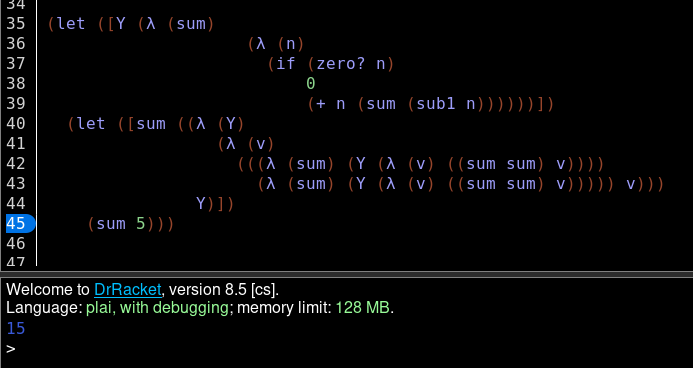
\includegraphics[scale=0.3]{./Sum-Y.png}
  \caption{Ejecución de la función dada.}
\end{figure}

Para esta función, tenemos una definición interna que realiza una recursión mutua,
la ejecución tiene que reducir las lambdas a su forma normal (en este caso siempre
es un valor numérico) y luego pasarselas a la función anterior o siguiente en el orden.
\newpage
%%%%%%%%%%%%%%%%%%%%%%%%%%%%%      Inciso C        %%%%%%%%%%%%%%%%%%%%%%%%%%%%%%%%%
\item Modifica la función usando el Combinador de Punto Fijo Z. Prueba la expresión en 
el intérprete de \code{Racket} y con base en la respuesta obtenida, explica el proceso que 
siguió el intérprete para llegar a ésta. Anexa una captura de pantalla del intérprete 
de \code{Racket} al probar la expresión.

\begin{figure}[h]
  \centering
  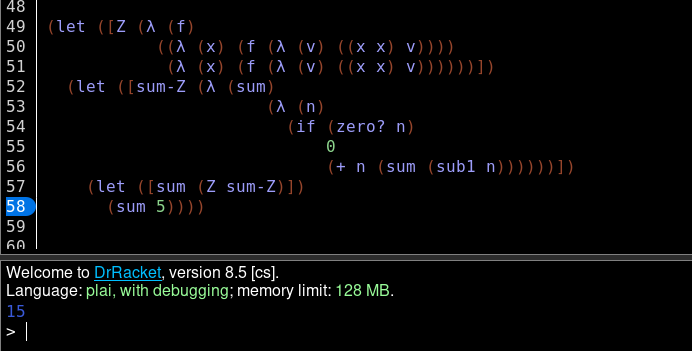
\includegraphics[scale=0.3]{./Sum-Z.png}
  \caption{Ejecución de la función dada.}
\end{figure}

Como en el ejercicio anterior, en la línea 27 se encuentra la modificación
que vuelve a esta función en un combinador de punto fijo Z. Inicialmente
reduce las lambdas a sus formas normales y ejecuta ambas funciones de manera
\textit{mutuamente recursiva} hasta llegar al valor deseado.
\end{enumerate}
